\documentclass[a4 paper]{article}
% Set target color model to RGB
\usepackage[inner=2.0cm,outer=2.0cm,top=2.5cm,bottom=2.5cm]{geometry}
\usepackage{setspace}
\usepackage[rgb]{xcolor}
\usepackage{verbatim}
\usepackage{amsmath}
\usepackage{subcaption}
\usepackage{amsgen,amsmath,amstext,amsbsy,amsopn,tikz,amssymb,tkz-linknodes}
\usepackage{fancyhdr}
\usepackage[colorlinks=true, urlcolor=blue,  linkcolor=blue, citecolor=blue]{hyperref}
\usepackage[colorinlistoftodos]{todonotes}
\usepackage{rotating}
%\usetikzlibrary{through,backgrounds}
\hypersetup{%
pdfauthor={},%
pdftitle={Homework},%
pdfkeywords={Tikz,latex,bootstrap,uncertaintes},%
pdfcreator={PDFLaTeX},%
pdfproducer={PDFLaTeX},%
}
%\usetikzlibrary{shadows}
% \usepackage[francais]{babel}
\usepackage{booktabs}
\newcommand{\ra}[1]{\renewcommand{\arraystretch}{#1}}

\newtheorem{thm}{Theorem}[section]
\newtheorem{prop}[thm]{Proposition}
\newtheorem{lem}[thm]{Lemma}
\newtheorem{cor}[thm]{Corollary}
\newtheorem{defn}[thm]{Definition}
\newtheorem{rem}[thm]{Remark}
\numberwithin{equation}{section}

\newcommand{\homework}[6]{
   \pagestyle{myheadings}
   \thispagestyle{plain}
   \newpage
   \setcounter{page}{1}
   \noindent
   \begin{center}
   \framebox{
      \vbox{\vspace{2mm}
    \hbox to 6.28in { {\bf CS 5691:~ Pattern Recognition and Machine Learning \hfill {\small (#2)}} }
       \vspace{6mm}
       \hbox to 6.28in { {\Large \hfill #1  \hfill} }
       \vspace{6mm}
       \hbox to 6.28in { {\it Instructor: {\rm #3} \hfill Name: {\rm #5}}}
       %\hbox to 6.28in { {\it TA: #4  \hfill #6}}
      \vspace{2mm}}
   }
   \end{center}
   \markboth{#5 -- #1}{#5 -- #1}
   \vspace*{4mm}
}

\newcommand{\problem}[2]{~\\\fbox{\textbf{Problem #1}}\hfill (#2 points)\newline\newline}
\newcommand{\subproblem}[1]{~\newline\textbf{(#1)}}
\newcommand{\D}{\mathcal{D}}
\newcommand{\Hy}{\mathcal{H}}
\newcommand{\VS}{\textrm{VS}}
\newcommand{\solution}{~\newline\textbf{\textit{(Solution)}} }
\newcommand{\comment}[1]{}
\newcommand{\bbF}{\mathbb{F}}
\newcommand{\bbX}{\mathbb{X}}
\newcommand{\bI}{\mathbf{I}}
\newcommand{\bX}{\mathbf{X}}
\newcommand{\bY}{\mathbf{Y}}
\newcommand{\bepsilon}{\boldsymbol{\epsilon}}
\newcommand{\balpha}{\boldsymbol{\alpha}}
\newcommand{\bbeta}{\boldsymbol{\beta}}
\newcommand{\0}{\mathbf{0}}

\begin{document}
\homework{Programming Assignment 1}{Due: 14/03/20}{L.A. Prashant}{}{Arvind Menon EP17B017 Ishan Sabane ED17B013}


\problem{1: Bayes Classifiers }{20}
\subproblem{a} For Dataset 1:
\begin{table}[h!]
\centering
 \begin{tabular}{|c|c|c|c|c|} 
 \hline
 Model & Training Accuracy & Test Accuracy \\ [0.5ex] 
 \hline
1 & 97.3888 \% & 97.1111 \% \\
2 & 97.3888 \% & 97.1111 \% \\
3 & 97.3888 \% & 97.1111 \% \\
4 & 97.3888 \% & 97.1111 \% \\
5 & 97.3888 \% & 97.1111 \% \\

\hline
\end{tabular}
\caption{Table of classification accuracies for all the models on training data and test data }
\end{table}

For Dataset 2
\begin{table}[h!]
\centering
 \begin{tabular}{|c|c|c|c|c|} 
 \hline
 Model & Training Accuracy & Test Accuracy \\ [0.5ex] 
 \hline
1 & 87.4166\% &  86.7777\% \\
2 & 89.3611\% &  87.6666\% \\
3 & 90.4722\% &  89.4444\% \\ 
4 & 89.0833\%  & 87.1111\% \\
5 & 91.4444\% &  91.0\% \\

\hline
\end{tabular}
\caption{Table of classification accuracies for all the models on training data and test data }
\end{table}
\section{Inference}
\begin{itemize}
\item [1] Dataset 1 gives the same accuracy for each model because the data for each class is very well separated making it easier to classify points to each of the classes and showing lesser dependence on the covariance matrix used for each of the classes, as long as you estimate the mean properly.
\item [2]From the above tables we can clearly see that model 5 or (e) is the best model. This can also be concluded theoretically by simply observing that model 5 has the least number of constraints on the class Covariance matrices out of all the models allowing it to make the most accurate classifications.

\end{itemize}
\newpage
\subproblem{b} 
\begin{figure}[!htb]
    \centering
    \begin{minipage}{0.50\textwidth}
        \centering
        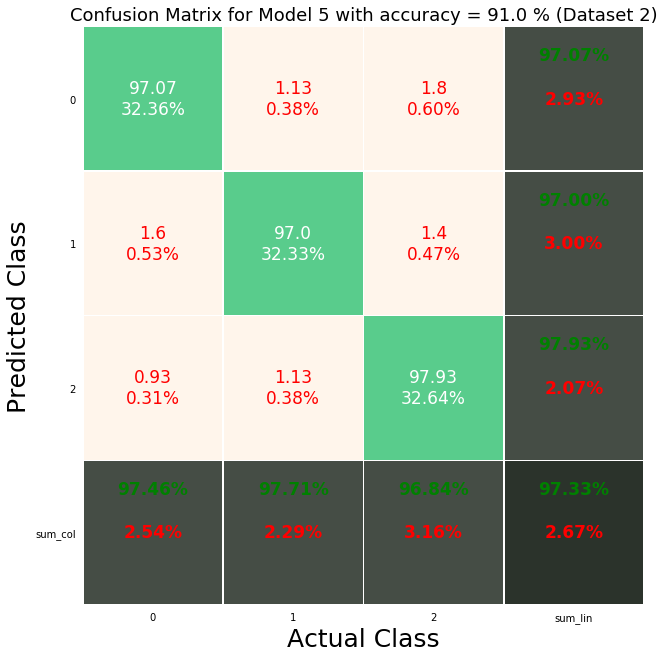
\includegraphics[width=1\textwidth]{cm1.png} \\
        \caption{Confusion Matrix for Dataset 1}
    \end{minipage}\hfill
    \begin{minipage}{0.50\textwidth}
        \centering
        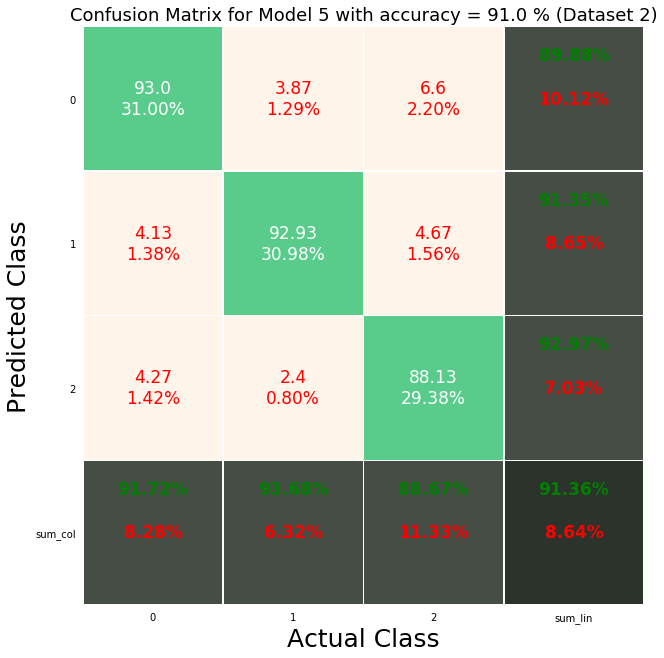
\includegraphics[width=1\textwidth]{cm2.png}\\
        \caption{Confusion Matrix for Dataset 2}
    \end{minipage}
    \label{fig:l}
\end{figure}


\subproblem{c} 
\begin{figure}[!htb]
    \centering
    \begin{minipage}{0.50\textwidth}
        \centering
        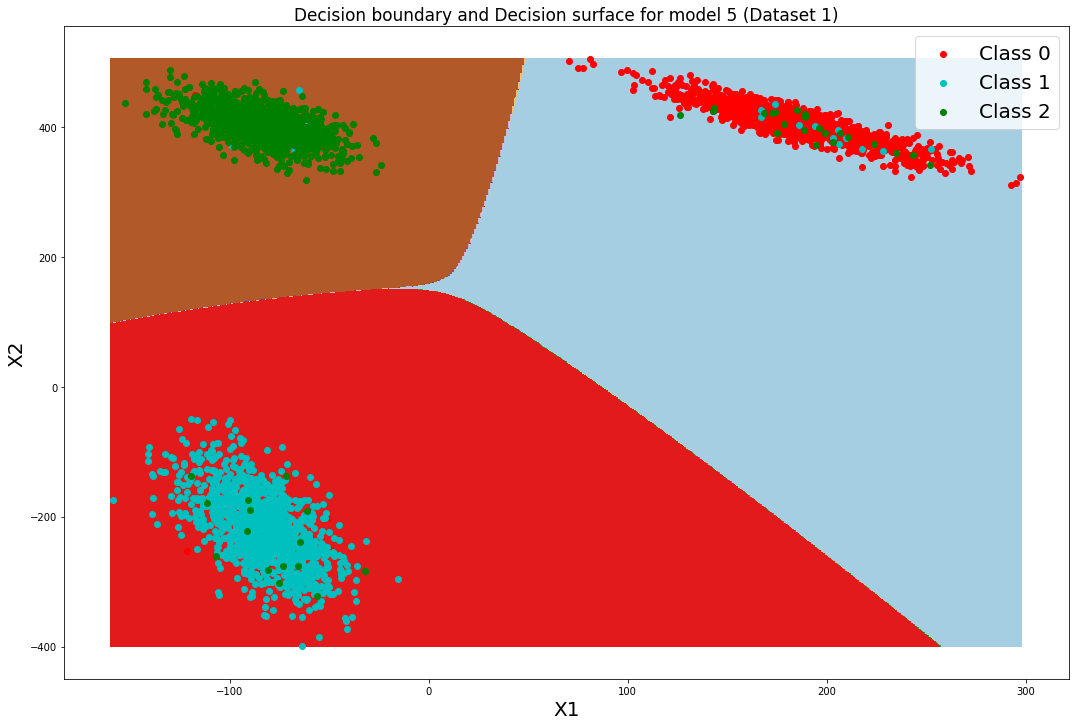
\includegraphics[width=1\textwidth]{decision_boundary1.png} \\
        \caption{Decision boundary for Dataset 1}
    \end{minipage}\hfill
    \begin{minipage}{0.50\textwidth}
        \centering
        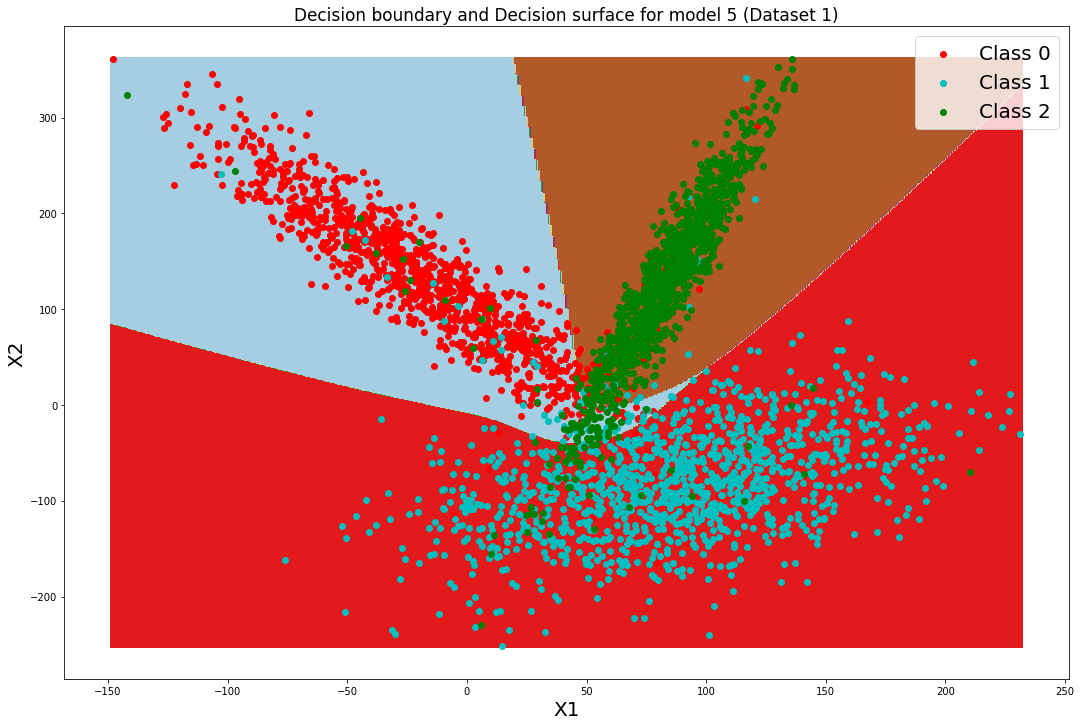
\includegraphics[width=1\textwidth]{decision_boundary2.png}\\
        \caption{Decision boundary for Dataset 2}
    \end{minipage}
    \label{fig:l}
\end{figure}

The decision boundaries clearly show the difference in the distributions of the datasets and explains why the trend in the accuracy table was very different. \\


\newpage
\subproblem{d} 
\begin{figure}[!htb]
    \centering
    \begin{minipage}{0.50\textwidth}
        \centering
        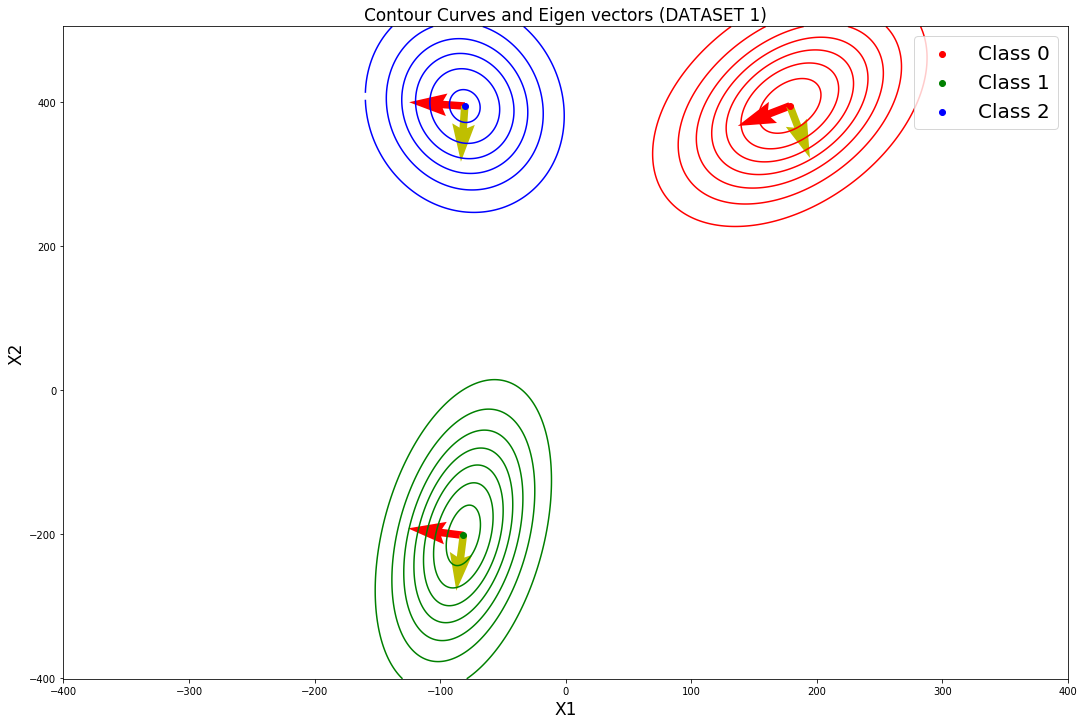
\includegraphics[width=1\textwidth]{eig1.png} \\
        \caption{Contour plot and eigenvectors for Dataset 1}
    \end{minipage}\hfill
    \begin{minipage}{0.50\textwidth}
        \centering
        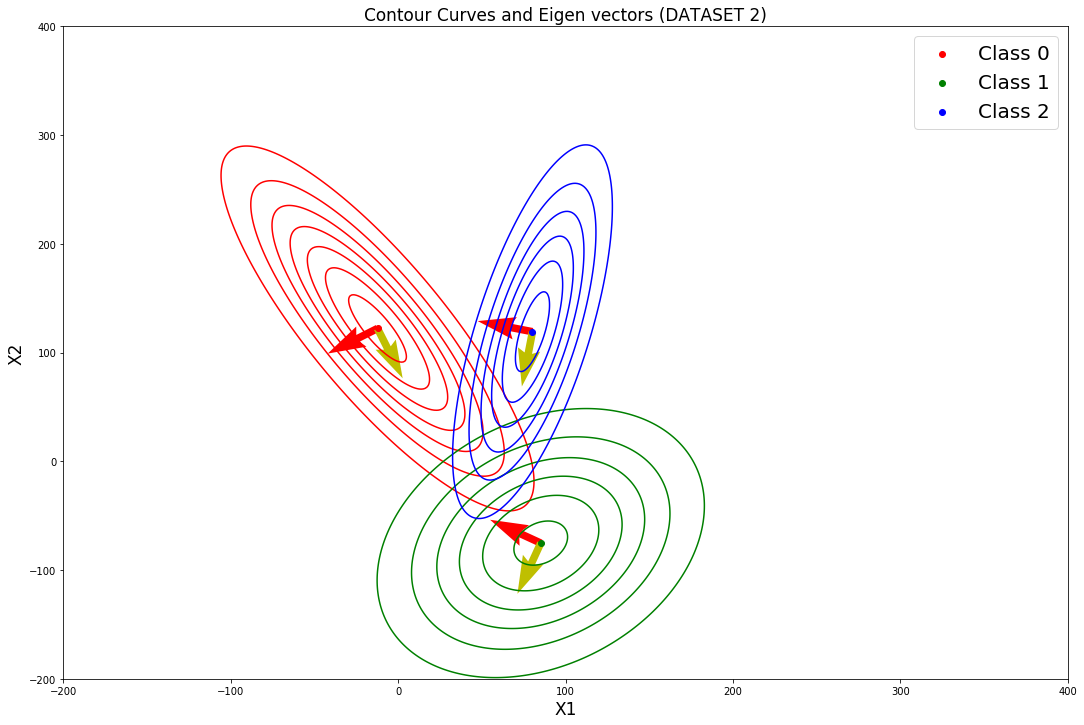
\includegraphics[width=1\textwidth]{eig2.png}\\
        \caption{Contour plot and eigenvectors for Dataset 2}
    \end{minipage}
    \label{fig:l}
\end{figure}

% Comment: In the objective, we wrote ``Practice writing proofs'' but this is rather simple and not very rigorous?


\problem{2: Bayesian Estimation of one dimension Guassian dataset}{4}

\subproblem{a}
$(\sigma = 3.8633 , \mu_{sample} = 0.95427417)$

\subproblem{b} 
 Estimate $\sigma$ by assuming that $\mu_0 = -1$. \\
\begin{equation}
    \sigma = \frac{\sum_{i=1}^{N}(x_i-\mu_n)^2}{N}
\end{equation}
\begin{table}[h!]
\centering
 \begin{tabular}{|c|c|c|c|c|} 
 \hline
 n & $(\frac{\sigma}{\sigma_0})^2$ = 0.1 & $(\frac{\sigma}{\sigma_0})^2$ = 1 & $(\frac{\sigma}{\sigma_0})^2$ = 10 & $(\frac{\sigma}{\sigma_0})^2$ = 100 \\ [0.5ex] 
 \hline
10	& 2.9520 &  2.9240 & 3.5480 & 5.4504\\
100	& 3.2623 &  3.2594 & 3.2615 & 4.0376\\
1000 & 3.8109 &  3.8108 & 3.8101 & 3.8317\\

\hline
\end{tabular}
\caption{Estimate of $\sigma$ from $\mu_n$ for 12 different cases }
\end{table}

Observations :
\begin{itemize}
\item As n increases the distribution shifts more towards the sample mean rather than $\mu_0$
\item As $(\frac{\sigma}{\sigma_0})^2$ decreases the distribution becomes narrower and closer to the sample mean of the distribution
\end{itemize}

\newpage
\begin{equation}
    \mathcal{P}(x|D) \sim N(\mu_n, \sigma^2 + \sigma_n^2) 
\end{equation}
\begin{figure}[!htb]
    \centering
    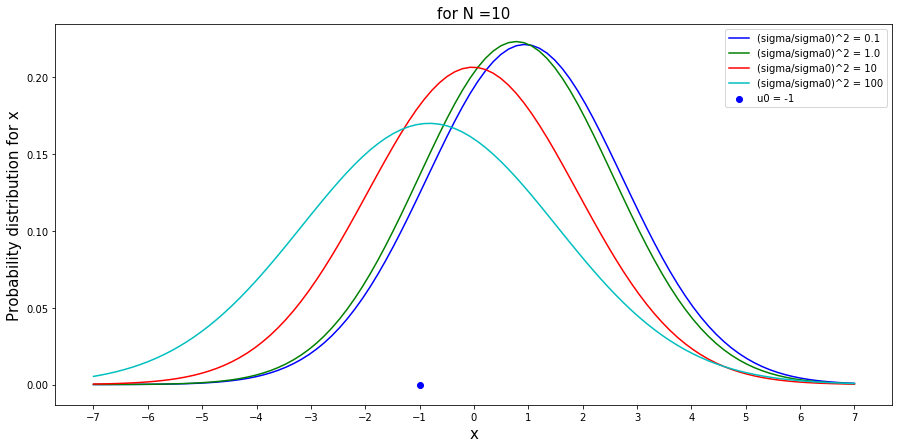
\includegraphics[width=0.7\textwidth]{gaussian(n=10).png}
    \caption{$\mathcal{P}(x/D)$ for n = 10}
    \label{fig:1}
\end{figure}

\begin{figure}[!htb]
    \centering
    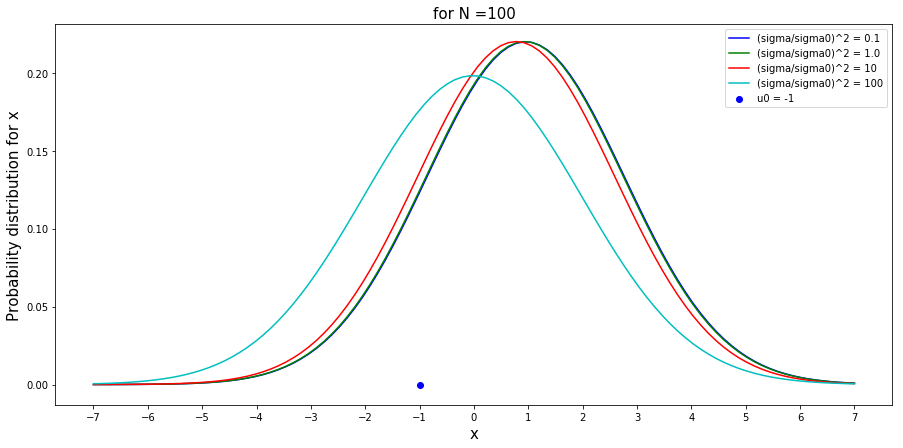
\includegraphics[width=0.7\textwidth]{gaussian(n=100).png}
    \caption{$\mathcal{P}(x/D) for n = 100$}
    \label{fig:2}
\end{figure}

\begin{figure}[!htb]
    \centering
    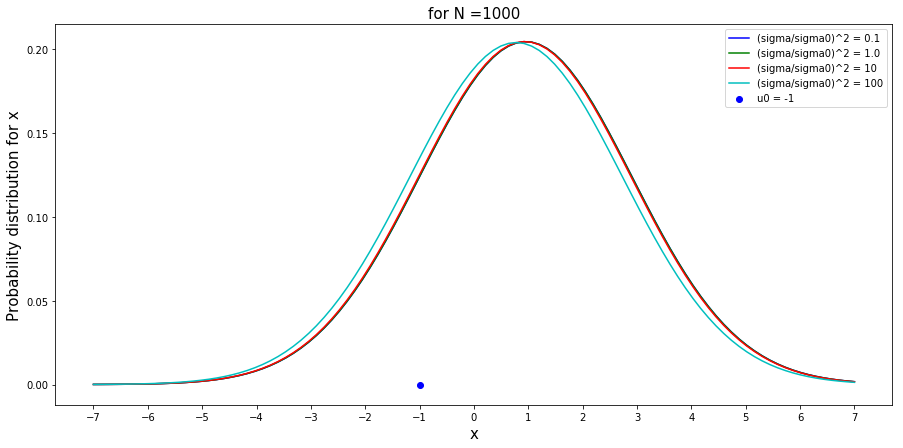
\includegraphics[width=0.7\textwidth]{gaussian(n=1000).png}
    \caption{$\mathcal{P}(x/D)$ for n = 1000}
    \label{fig:3}
\end{figure}


\newpage
\problem{3: Maximum Likelihood Estimation}{10 points}

\subproblem{a}

Estimated Mean = ( 0.50468154  1.76937047 -0.80748207)\\

Estimated Covariance Matrix =
\begin{bmatrix}
     4.03453523 & 1.83796218 &  -0.42437584\\
     1.83796218 & 10.26916473 & -4.51444933 \\
     -0.42437584 & -4.51444933 & 10.64430326 \\
\end{bmatrix}
\\



\subproblem{b}
We find the training error using new co-variance matrices $\Sigma_i(\alpha)$ found by the equation : \\
\begin{equation}
    \Sigma_i(\alpha)=\frac{(1-\alpha)n_i\Sigma_i + \aplha n\Sigma}{(1-\alpha)n_i + \alpha n}
\end{equation}

\begin{figure}[!htb]
    \centering
    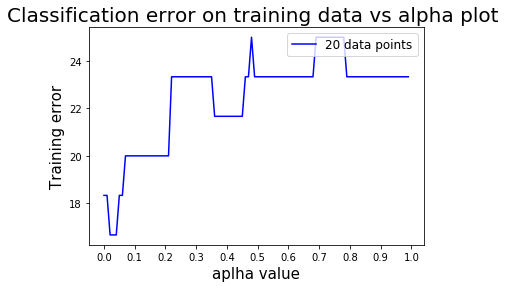
\includegraphics[width=0.7\textwidth]{MLE_train.png}
    \caption{Training error $(\%)$ vs $\alpha$}
    \label{fig:2}
\end{figure}

\subproblem{c}
Data points from each class = 50

\begin{figure}[!htb]
    \centering
    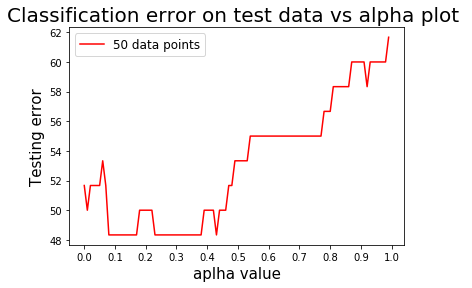
\includegraphics[width=0.7\textwidth]{MLE_test.png}
    \caption{Testing error $(\%)$ vs $\alpha$}
    \label{fig:2}
\end{figure}


\clearpage
\problem{4: Singular Value Decomposition}{8 points}
The Frobenius Norm of a Matrix  $A_{mxn}$  is given by the equation:\\
\begin{equation}
    \|\mathbf{A} _{F}\| = \sqrt{\mathop{\sum_{i=i}^{m}\sum_{j=1}^{n}}{a_{ij}^{2}}}
\end{equation}\\
\bigskip
\textbf{Part A}: 100x100 Matrix With Highly Co-correlated Adjacent Entries.\\
The highly co-related matrix A is created as follows:\\
$(1)$ A column Vector consisting of 100 random values between $(0,1)$ is generated.\\
$(2)$ This column Vector is multiplied by a random value between $(0,1)$ and Gaussian noise of very low magnitude is added.\\
$(3)$ This Column Matrix is assigned as the first column of the 100x100 matrix.\\
$(4)$ Above procedure is iterated to fill up all the 100 columns and then we get a highly co-related 100x100 matrix.\\
\begin{table}[h!]
\centering
 \begin{tabular}{|c|c|} 
 \hline
 Matrix  & Frobenius Norm \\ [0.5ex] 
\hline
A                             &  38.537\\
Top 10\% Singular Vectors     &  38.223\\
Random 10\% Singular Vectors  &  1.622\\
\hline
\end{tabular}
\caption{Frobenius Norm Using Singular Vectors}
\end{table}
\subproblem{a} The Frobenius Norm of the generated matrix is :38.537
\subproblem{b} The Top 10\% Singular Vectors Capture 99.425\% of the Frobenius Norm of Matrix  A.
\subproblem{c} Random 10\% Singular Vectors Capture 4.211\% of the Frobenius Norm of Matrix A.
\subproblem{d} Plot of Percentage of Data Captured Vs Number of Singular Vectors Required.\\
\begin{figure}[!htb]
    \centering
    \begin{minipage}{0.49\textwidth}
        \centering
        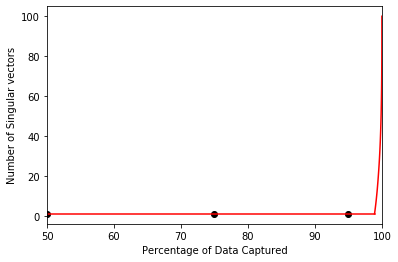
\includegraphics[width=1\textwidth]{Highly coorelated 1.png} \\
         Plot With Required Data Points
    \end{minipage}\hfill
    \begin{minipage}{0.49\textwidth}
        \centering
        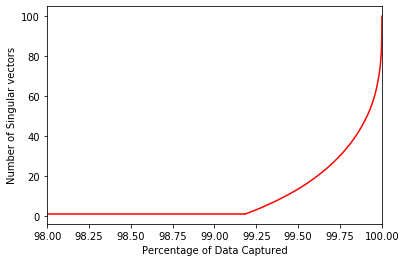
\includegraphics[width=1\textwidth]{Highly coorelated 2.png}\\
          Magnified Plot
    \end{minipage}
    \label{fig:l}
\end{figure}

\begin{table}[h!]
\centering
 \begin{tabular}{|c|c|} 
 \hline
Data Captured  & Number of Singular Vectors Required\\ [0.5ex] 
\hline
50\% &  1\\
75\% &  1\\
95\% &  1\\
\hline
\end{tabular}
\caption{Number of Singular Vectors To Capture Data}
\end{table}
\newpage
\subproblem{e} Observations:
\begin{itemize}
  \item As the Matrix has Highly Co-related Elements, it has one large eigenvalue which captures almost the whole matrix data .
  \item The random 10\% Singular Vectors may capture either very less matrix data if it does not have the topmost singular vector or almost all matrix data if it has the topmost singular vector.
  \item Exact 50\%, 75\%, 95\%  Matrix data cannot be captured because the first Singular Vector captures 99.1\% Matrix Data.  
\end{itemize}
\bigskip
\textbf{Part B:} 100x100 Matrix A With Statistically Independent Elements.\\

In order to eliminate the pseudo-randomness of the np.random.rand(), the following method is used to create a 100*100 Matrix with independent Elements:
\begin{itemize}
    \item A Matrix is created using np.random.rand(100,100).
    \item Then each element of the created Matrix is taken to be the mean of a Gaussian Distribution with SD=1.
    \item Each element of the matrix is replaced by the Gaussian output obtained. Some Gaussian Noise is added.
    \item The Matrix is scaled down such that all elements are between (0,1);
\end{itemize}
  
\begin{table}[h!]
\centering
 \begin{tabular}{|c|c|} 
 \hline
 Matrix  & Frobenius Norm \\ [0.5ex] 
\hline
A                             &  25.508\\
Top 10\% Singular Vectors     &  15.595\\
Random 10\% Singular Vectors  &  7.329\\
\hline
\end{tabular}
\caption{Frobenius Norm Using Singular Vectors}
\end{table}
\subproblem{a} The Frobenius Norm of the generated matrix A is 25.508.
\subproblem{b} The Top 10\% Singular Vectors Capture  61.139\% of the Data.
\subproblem{c} Random 10\% Singular Vectors Capture 28.734\% of the Data.
\subproblem{d} Plot of Percentage of Data Captured Vs Number of Singular Vectors Required.\\
\begin{figure}[!htb]
    \centering
    \begin{minipage}{0.49\textwidth}
        \centering
        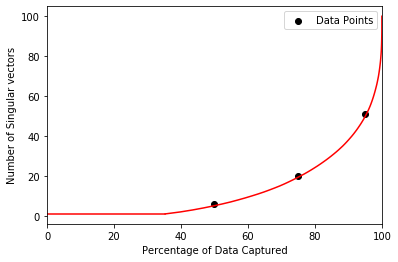
\includegraphics[width=1\textwidth]{SIndependent1.png} \\
         Plot With Required Data Points
    \end{minipage}\hfill
    \begin{minipage}{0.49\textwidth}
        \centering
        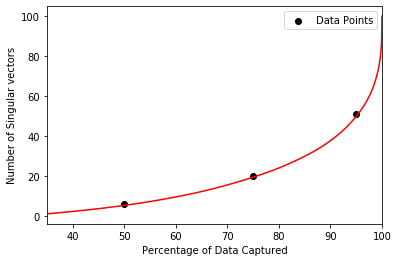
\includegraphics[width=1\textwidth]{SIndependent2.png}\\
          Magnified Plot
    \end{minipage}
    \label{fig:l}
\end{figure}
\begin{table}[h!]
\centering
 \begin{tabular}{|c|c|} 
 \hline
Data Captured & Number of Singular Vectors Required \\ [0.5ex] 
\hline
50\% &  6\\
75\% &  20\\
95\% &  51\\
\hline
\end{tabular}
\caption{Number of Singular Vectors To Capture Data}
\end{table}
\newpage
\subproblem{e} Observations:
\begin{itemize}
  \item As the Matrix has independent elements, there are multiple singular values of the similar magnitude. Hence many singular vectors are needed to capture considerable amount of Matrix Data. 
  \item The random 10\%  capture around 28-40\% Matrix Data. It depends on whether some of the top 10\% singular vectors are selected or not. 
  \item Half of the Singular vectors are required to capture 95\% Matrix Data.
\end{itemize}




\newpage
\problem{5: Principal Component Analysis}{10 Points}

\subproblem{a} The gray scale of the original image can be obtained using: cv2.IMREAD\_GRAYSCALE 
\begin{figure}[!htb]
    \centering
    \begin{minipage}{0.49\textwidth}
        \centering
        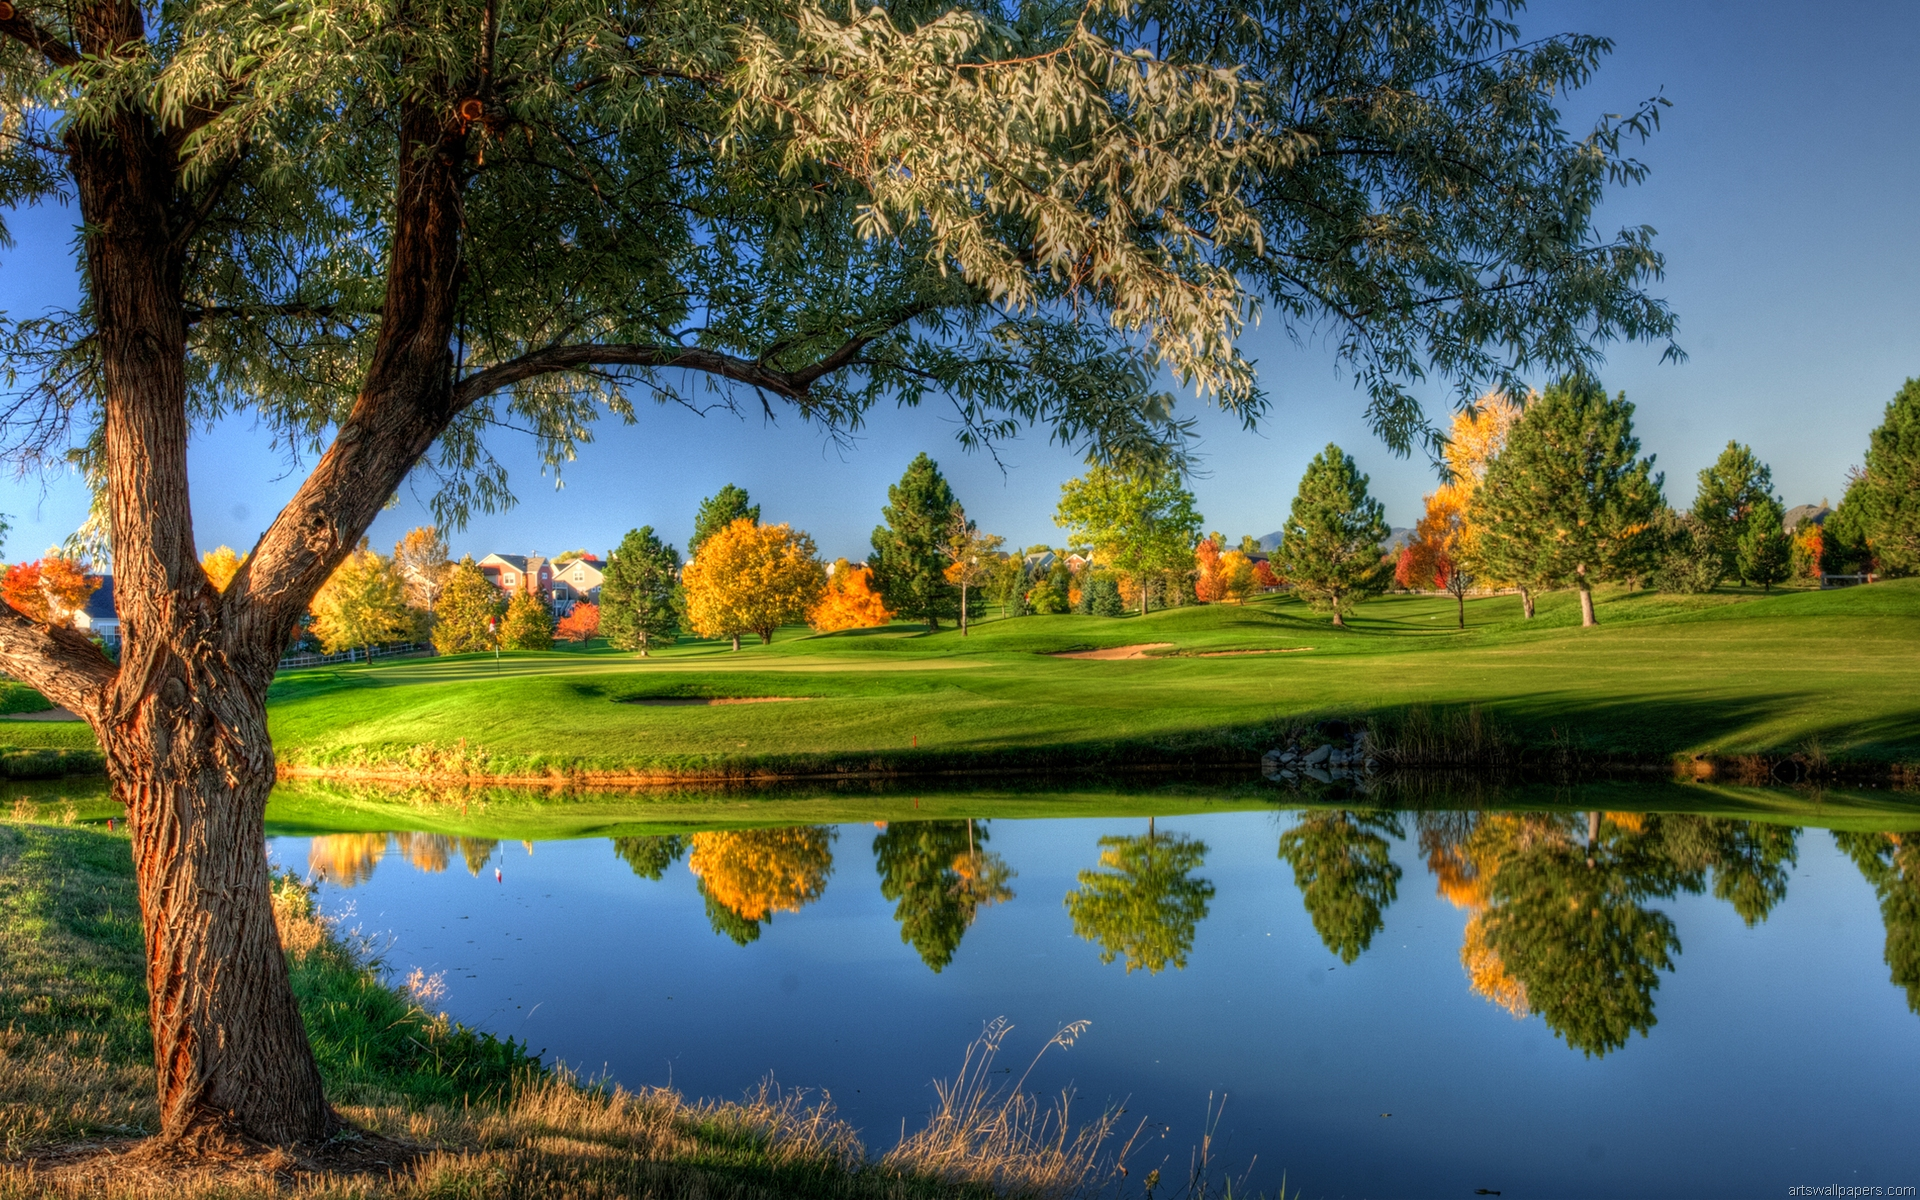
\includegraphics[width=1\textwidth]{17.jpg} \\
         Original Image
    \end{minipage}\hfill
    \begin{minipage}{0.49\textwidth}
        \centering
        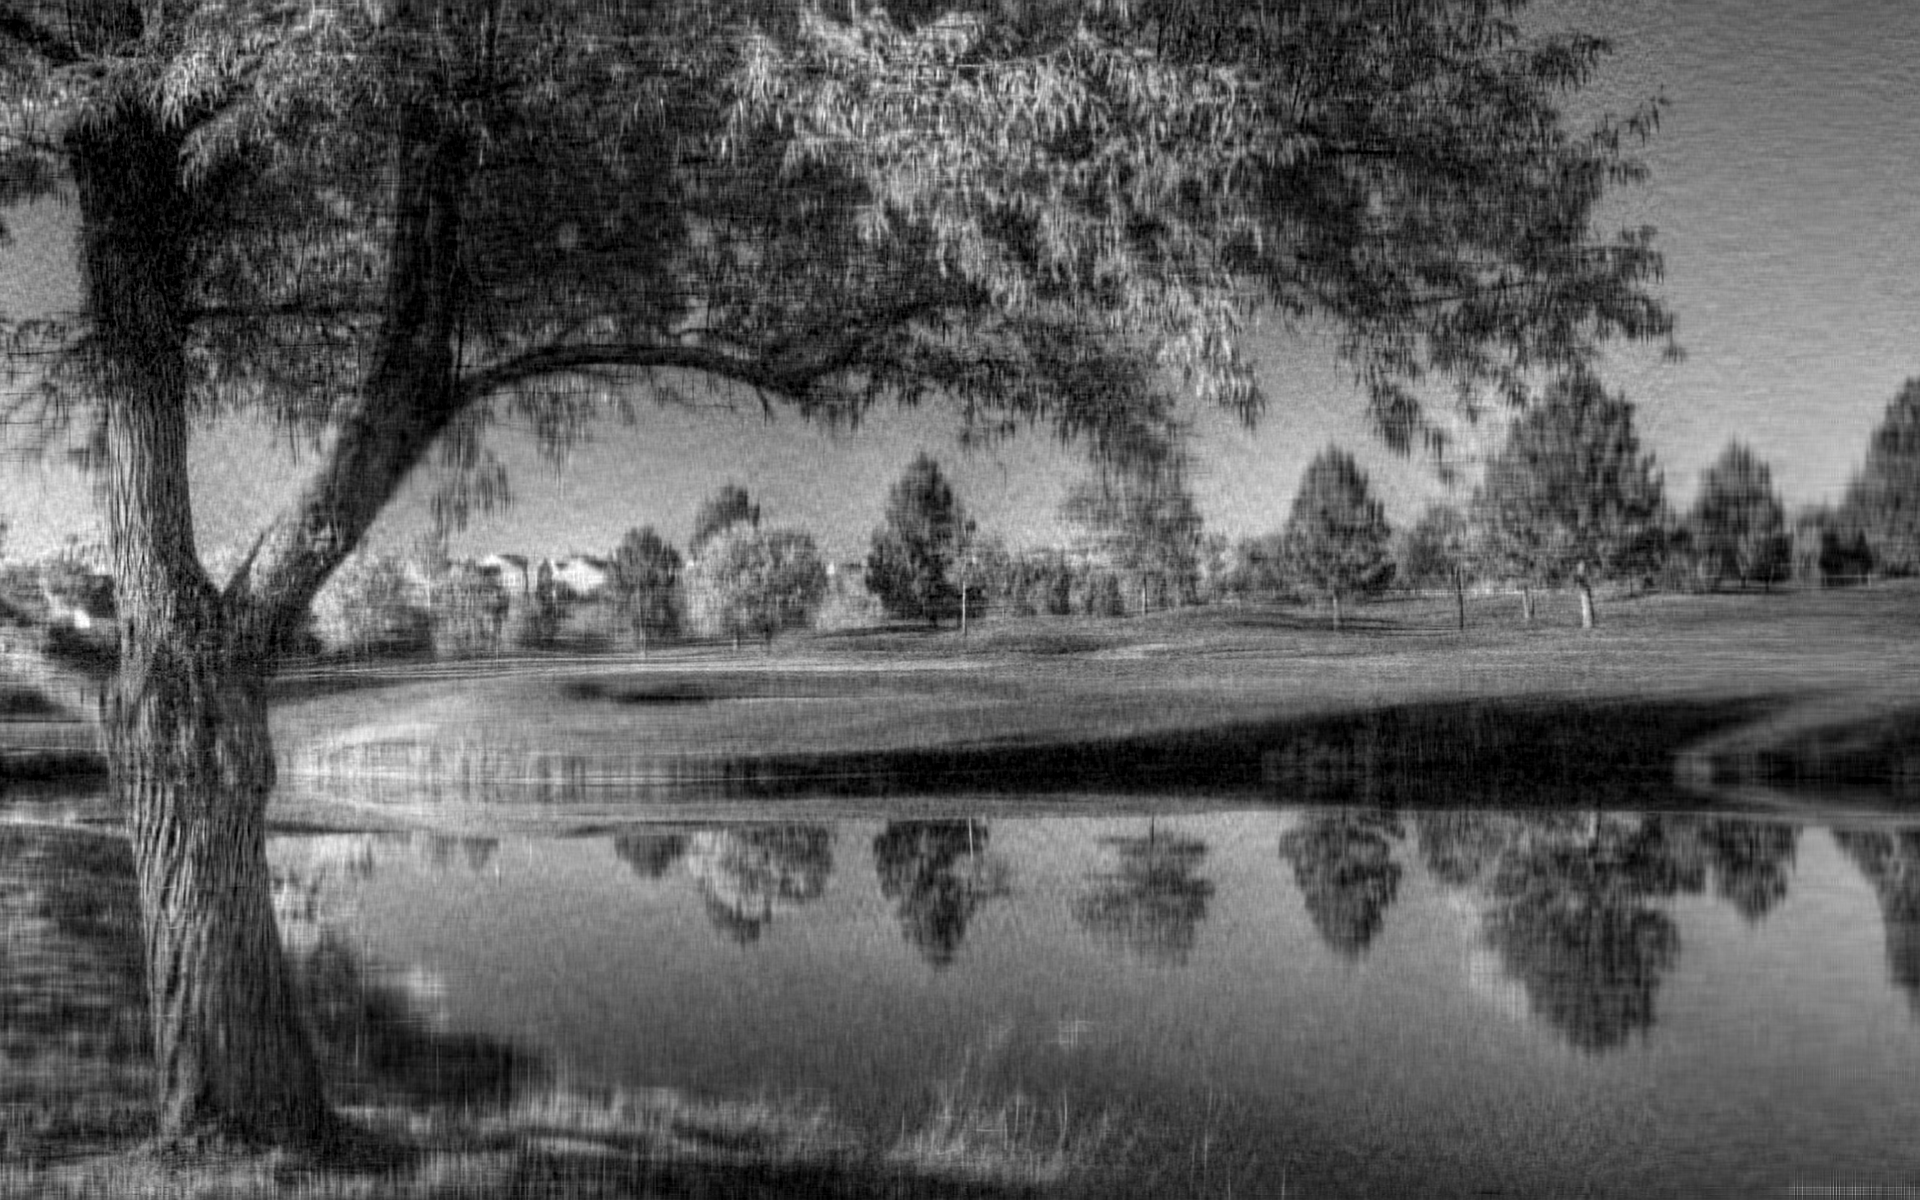
\includegraphics[width=1\textwidth]{grayscale.png}\\
         Gray-scale Image
    \end{minipage}
    \label{fig:l}
\end{figure}


\subproblem{b}Reconstructed and Error Images using top 10\% 25\% and 50\% Principal Components.\\

Top 10\% Principal Components.\\
\begin{figure}[!htb]
    \centering
    \begin{minipage}{0.49\textwidth}
        \centering
        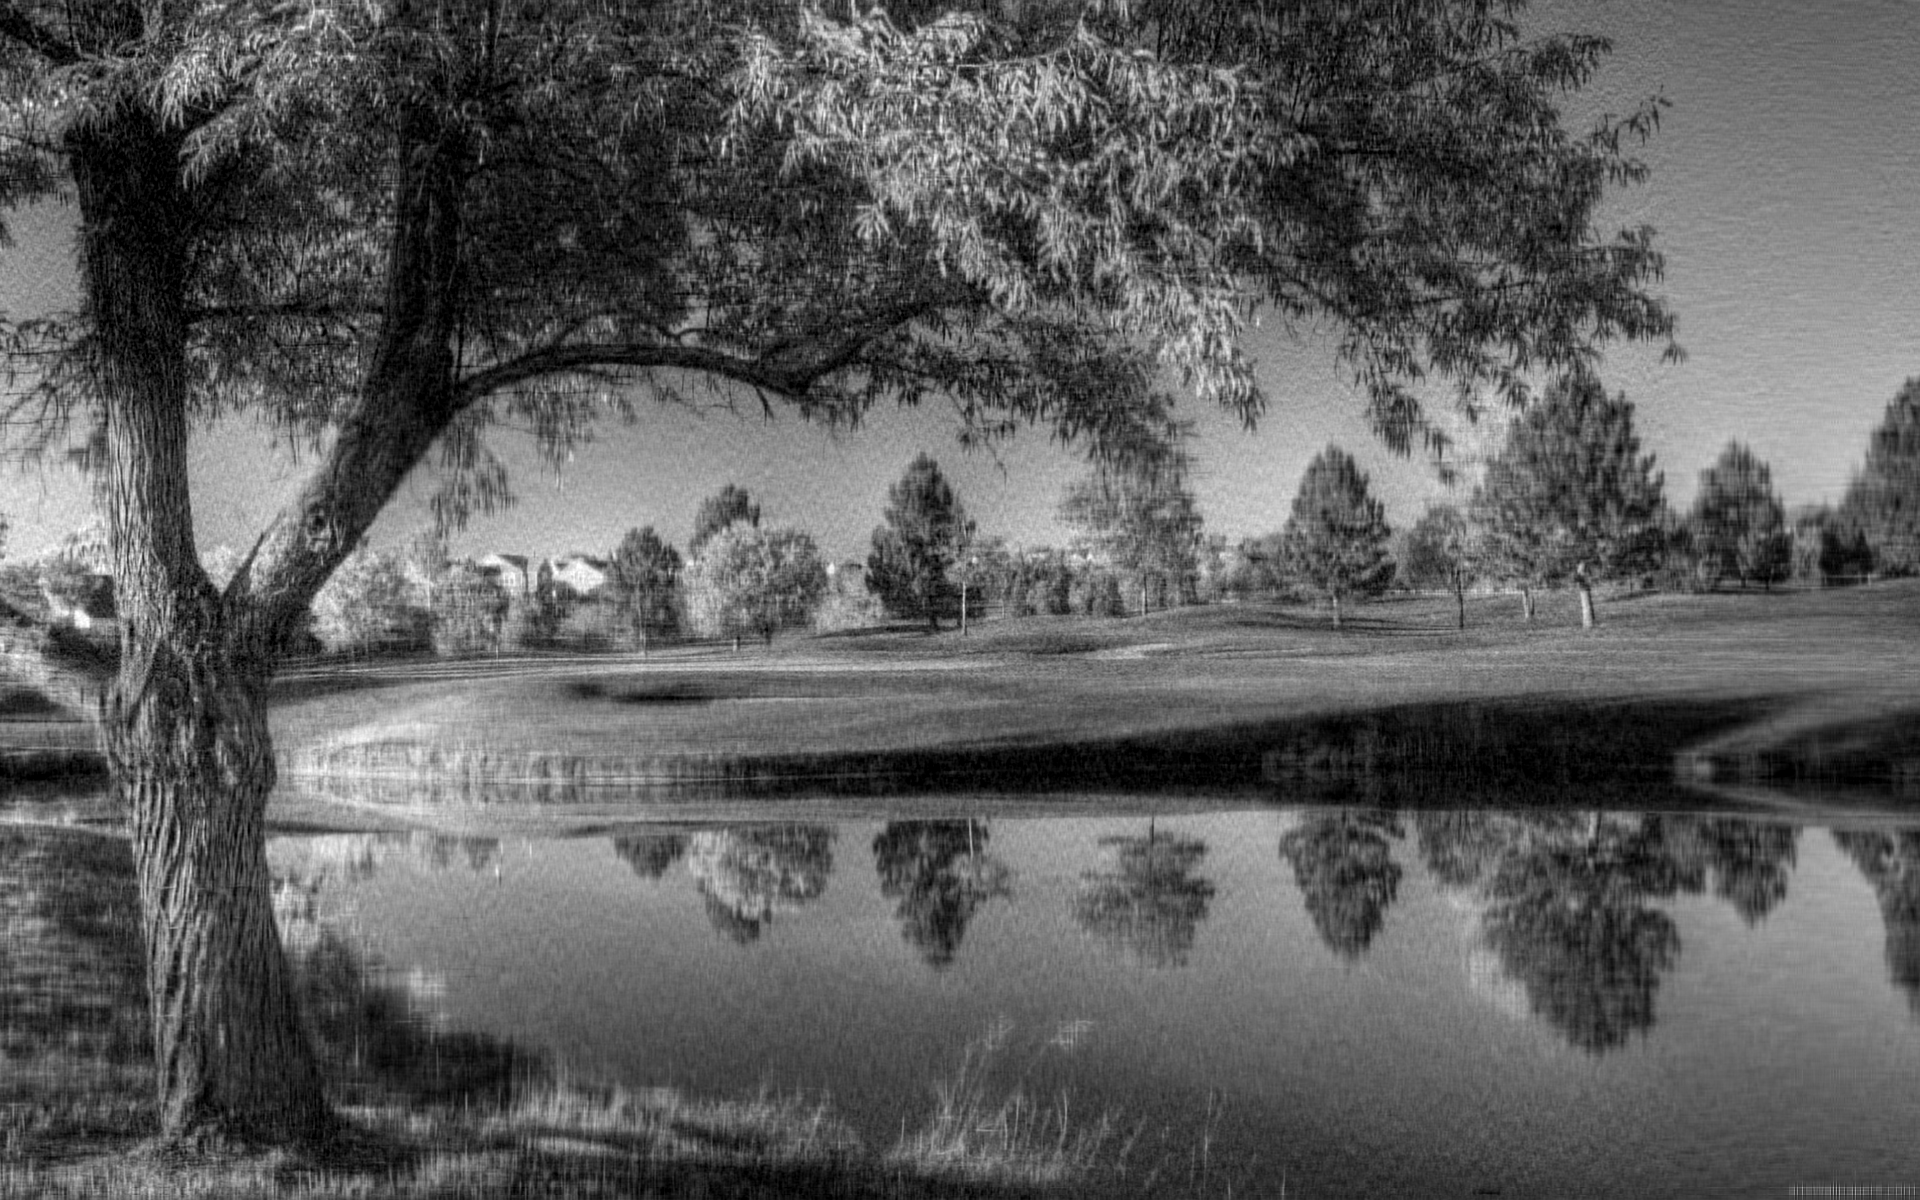
\includegraphics[width=1\textwidth]{R10.png} \\
         (a)Reconstructed Image
    \end{minipage}\hfill
    \begin{minipage}{0.49\textwidth}
        \centering
        
\includegraphics[width=1\textwidth]{E10.png}\\
         (b)Error Image
    \end{minipage}
    \label{fig:l}
\end{figure}

Top 25\% Principal Components.\\
\begin{figure}[!htb]
    \centering
    \begin{minipage}{0.49\textwidth}
        \centering
        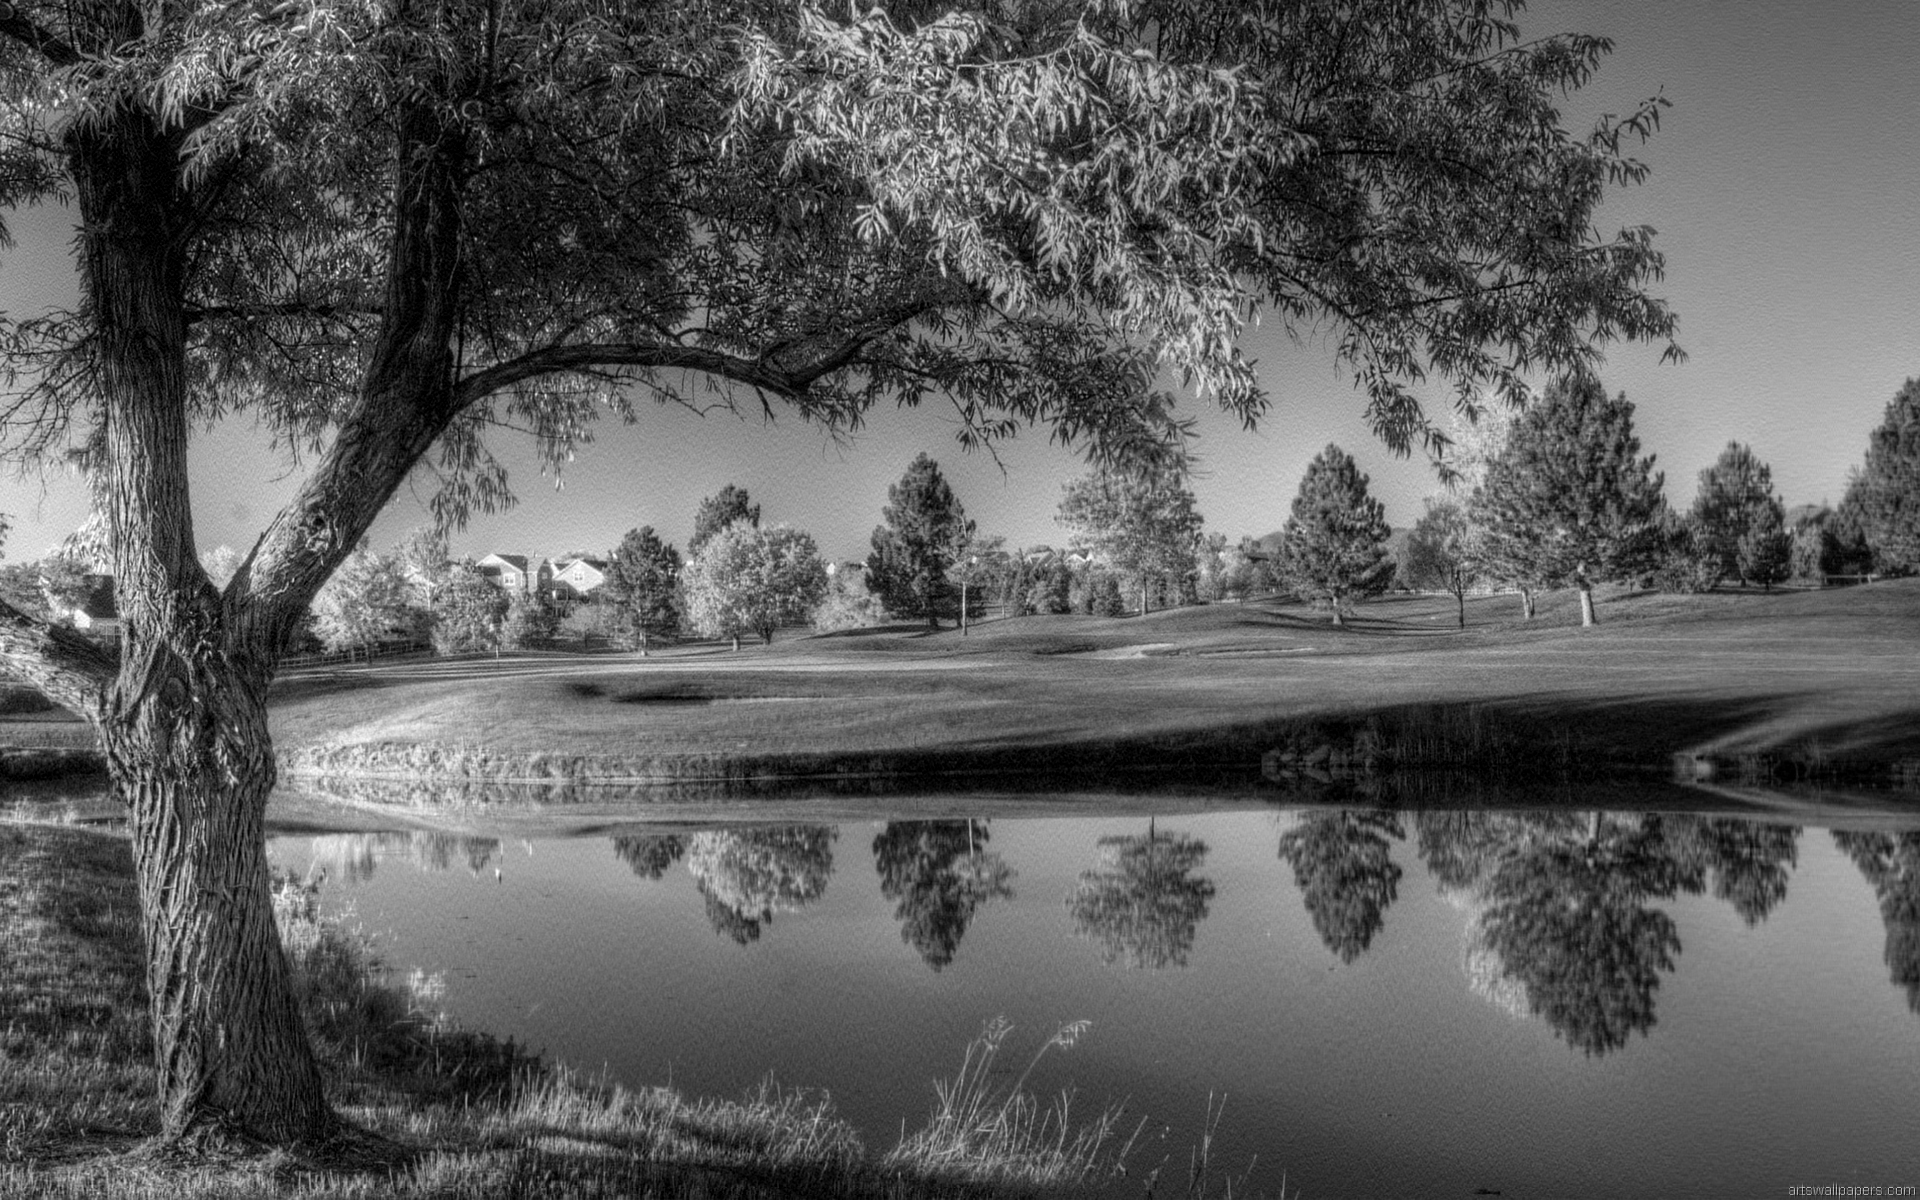
\includegraphics[width=1\textwidth]{R25.png} \\
         (c)Reconstructed Image
    \end{minipage}\hfill
    \begin{minipage}{0.49\textwidth}
        \centering
        
\includegraphics[width=1\textwidth]{E25.png}\\
         (d)Error Image
    \end{minipage}
    \label{fig:l}
\end{figure}

Top 50\% Principal Components.
\begin{figure}[!htb]
    \centering
    \begin{minipage}{0.49\textwidth}
        \centering
        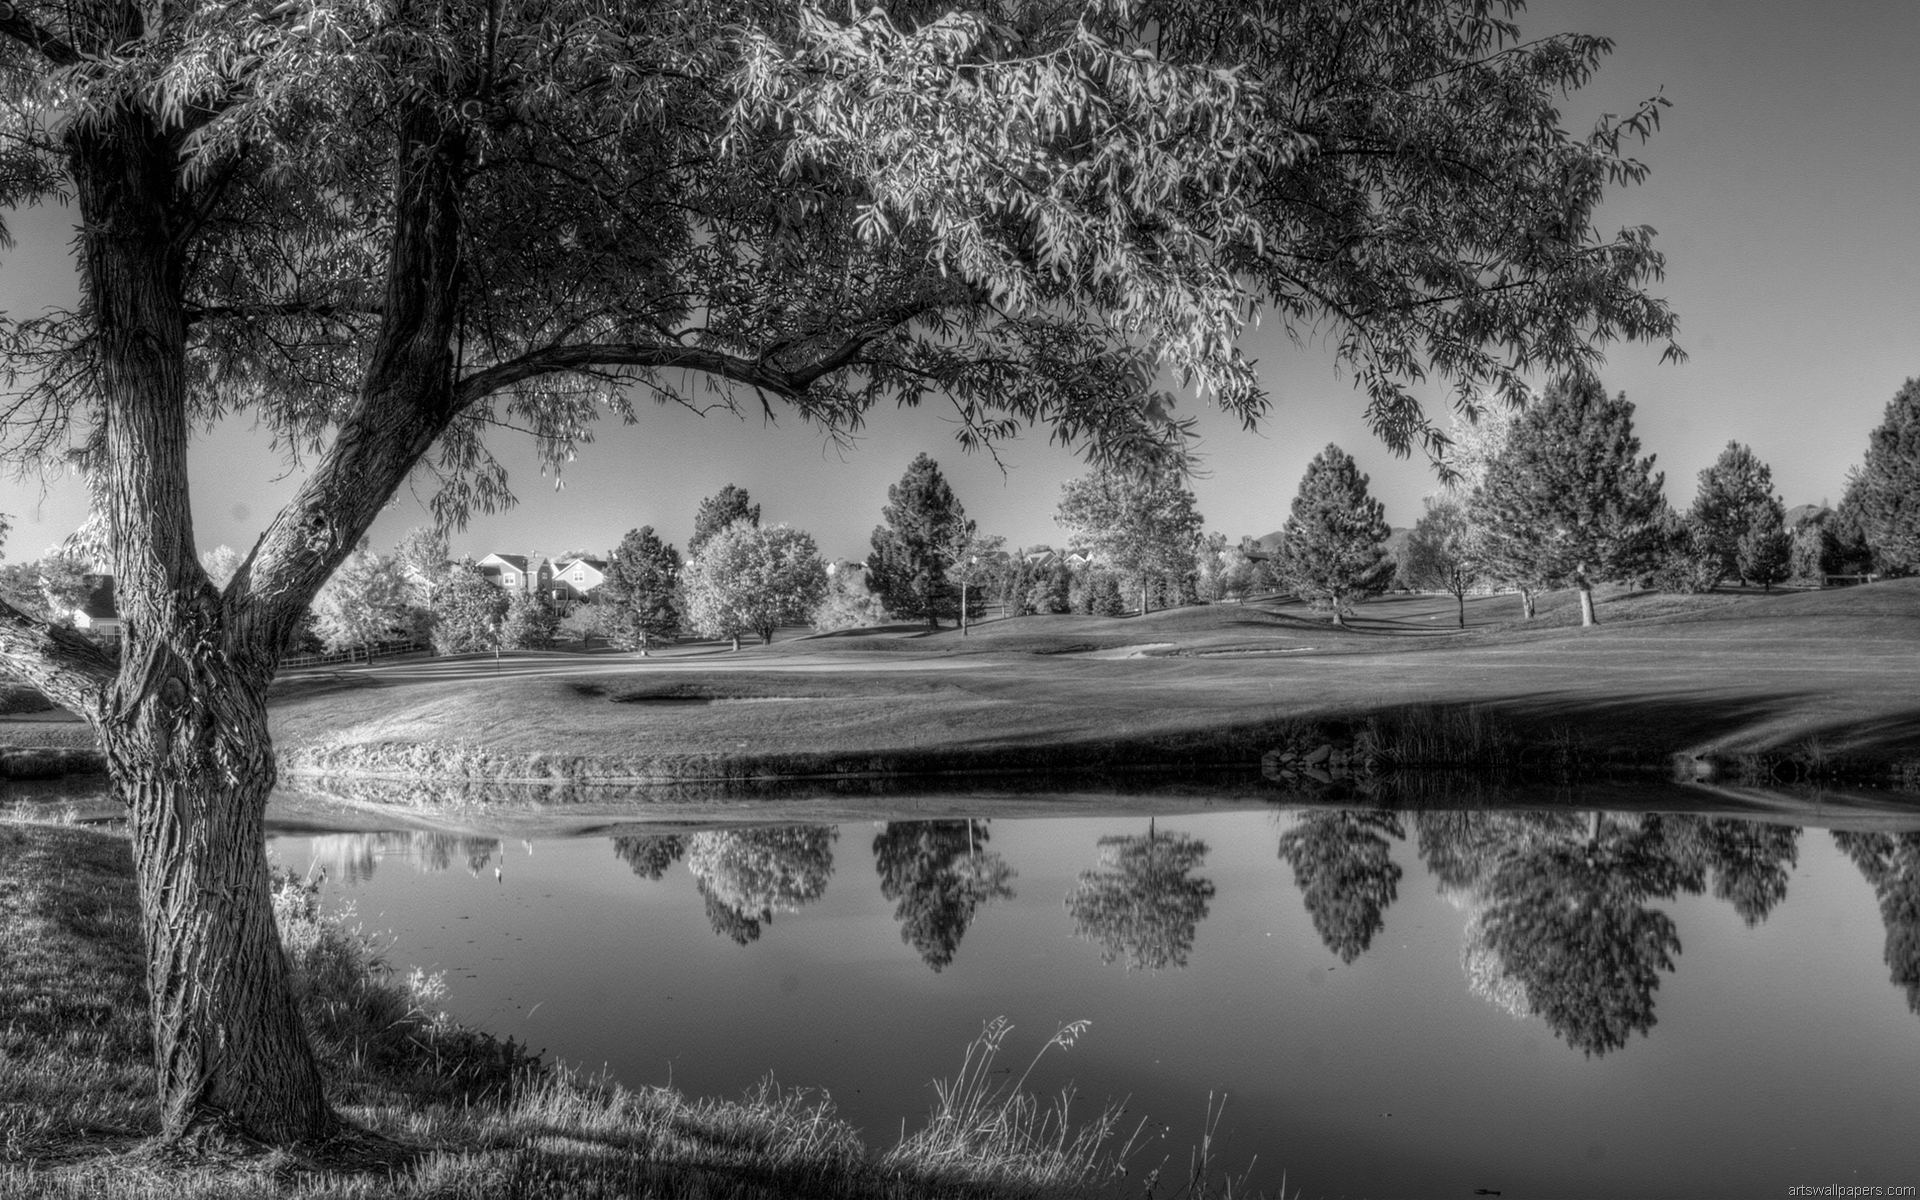
\includegraphics[width=1\textwidth]{R50.png} \\
         (e)Reconstructed Image
    \end{minipage}\hfill
    \begin{minipage}{0.49\textwidth}
        \centering
        
\includegraphics[width=1\textwidth]{E50.png}\\
        (f) Error Image
    \end{minipage}
    \label{fig:l}
\end{figure}

\subproblem{c} Random 10\% Principal Components.\\
\begin{figure}[!htb]
    \centering
    \begin{minipage}{0.49\textwidth}
        \centering
        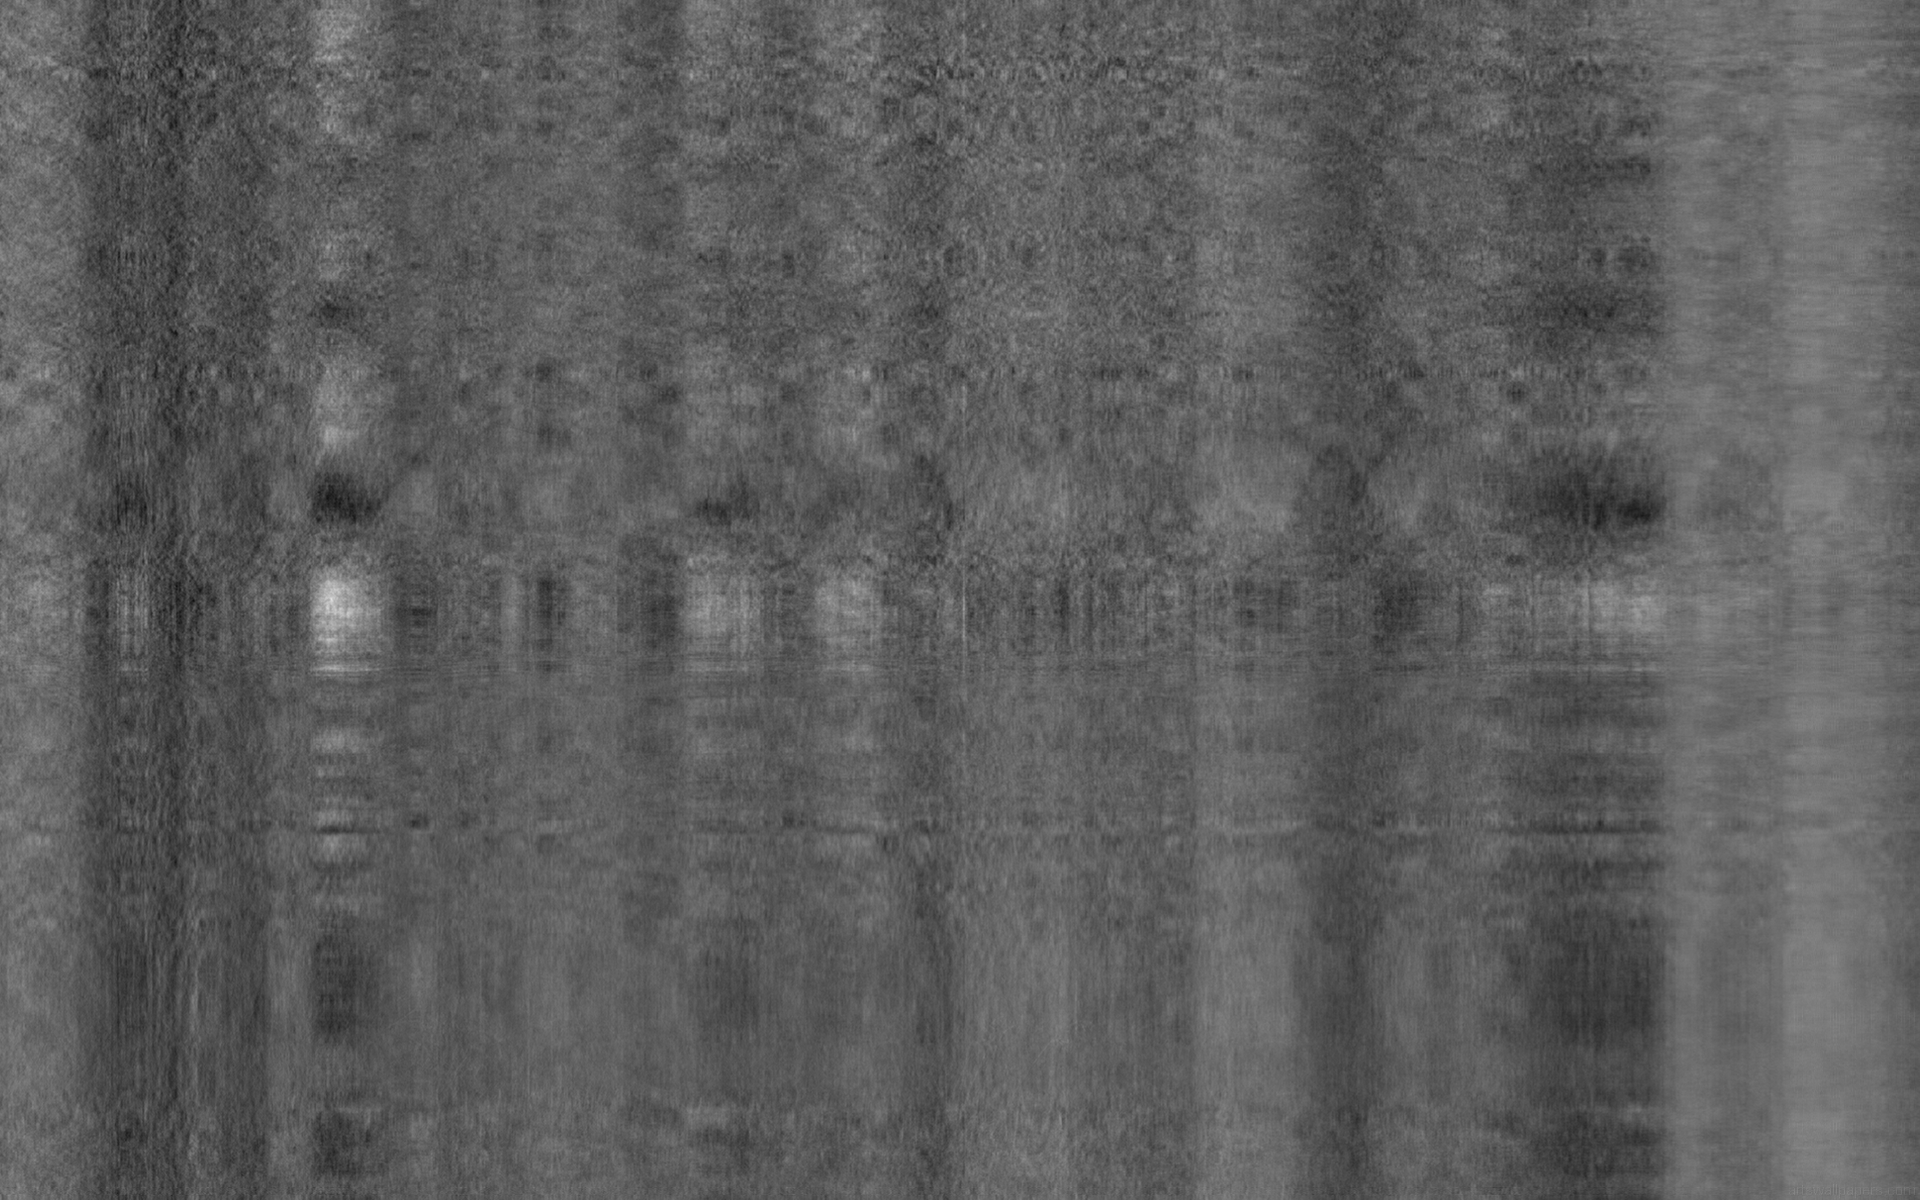
\includegraphics[width=1\textwidth]{Random10_R.png} \\
        (g) Reconstructed Image
    \end{minipage}\hfill
    \begin{minipage}{0.49\textwidth}
        \centering
        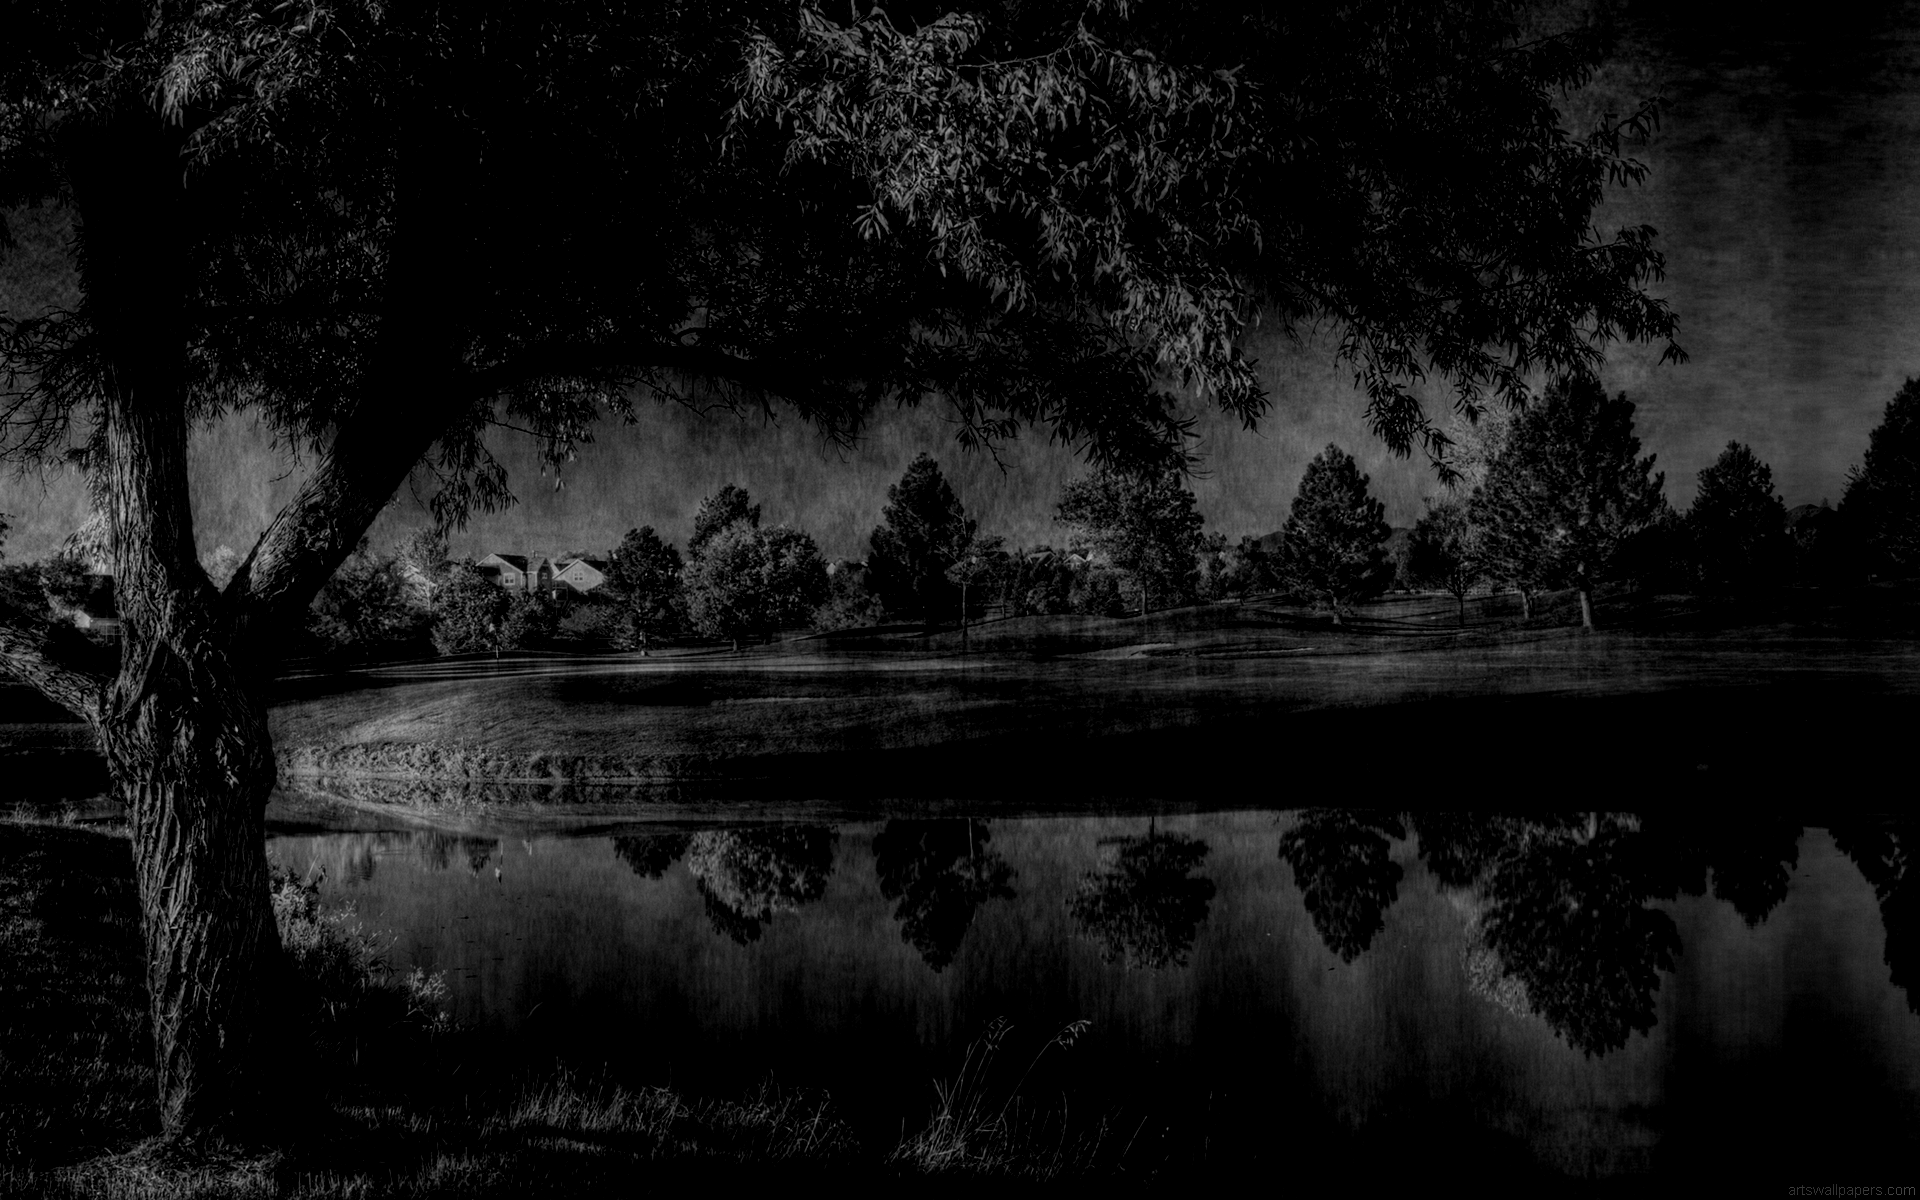
\includegraphics[width=1\textwidth]{Random10_E.png}\\
         (h)Error Image
    \end{minipage}
    \label{fig:l}
\end{figure}

\begin{equation}
    \text{Quality of Image(\%)} = \dfrac{\text{Frobenius Norm of Reconstructed Image}}{\text{Frobenius Norm of Original Image}}\times 100
\end{equation}\\
\begin{equation}
    \text{Reconstruction Error(\%)} = \dfrac{\text{Frobenius Norm of Error Image}}{\text{Frobenius Norm of Original Image}}\times 100
\end{equation}\\
\begin{table}[h!]
\centering
\begin{tabular}{|c|c|c|} 
\hline
Principal Components & Image Quality(\%) & Reconstruction Error(\%)\\ [0.5ex] 
\hline
Top 10\% & 99.14\%  & 13.055\% \\
Top 25\% & 99.75\% & 6.947\% \\
Top 50\% & 99.97\% & 2.4128\% \\
Random 10\%&55.20\%& 44.79\%\\
\hline
\end{tabular}
\caption{Image Quality and Reconstruction Error}
\end{table}
\begin{itemize}
  \item We can see from the above images (g) and (h) that the error image is actually better than the reconstructed image. Hence, the random 10\% Principal Components do not extract the required Image data and the important data is left out in the  error image.
  \item The probability of randomly choosing top 10\% Principal Components is negligible. Hence we must avoid Image Reconstruction using random Principal Components. 
\end{itemize}
. 


\newpage
\subproblem{d} Reconstruction Error Vs Top N\% Principal Components
\begin{figure}[!htb]
    \centering
        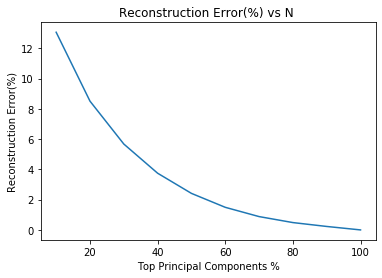
\includegraphics[width=0.5\textwidth]{Reconstruction vs N.png} \\
    
    \label{fig:l}
\end{figure}
\subproblem{e} Observations And Inferences:
\begin{itemize}
  \item Images reconstructed using more than Top 10\% Principal Components have excellent Image Quality.
  \item The Reconstruction error decreases exponentially with percentage of Principal Components used. 
  \item The Image can be compressed to 20-25\% without loss in Image Quality and with very low Reconstruction Error.
\end{itemize}




\newpage
\problem{6:Linear Model and Bias Variance}{10 Points}

The target function given is: 
\begin{equation}
   t = e^{\sin{(2*\Pi*x)}}+x 
\end{equation}
The value of x lies between (0,1) and some Gaussian noise is added to the target value. 
\subproblem{a} Linear Models for degrees 1,3,6,9 using 10 Data Points:
\begin{figure}[!htb]
    \centering
    \begin{minipage}{0.49\textwidth}
        \centering
        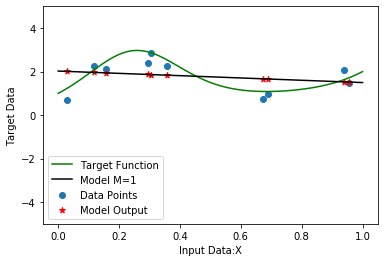
\includegraphics[width=1\textwidth]{M=1.png} \\
        (a) M=1
    \end{minipage}\hfill
    \begin{minipage}{0.49\textwidth}
        \centering
        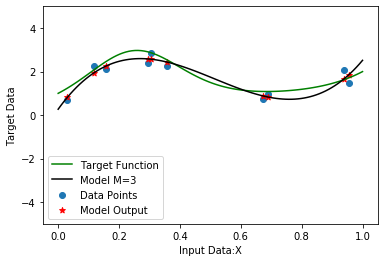
\includegraphics[width=1\textwidth]{M=3.png}\\
        (b) M=3
    \end{minipage}
    \label{fig:l}
\end{figure}
\begin{figure}[!htb]
    \centering
    \begin{minipage}{0.49\textwidth}
        \centering
        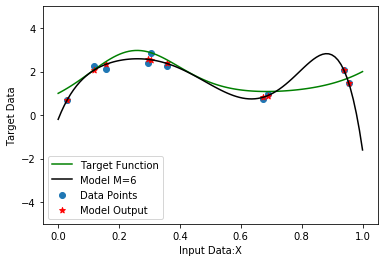
\includegraphics[width=1\textwidth]{M=6.png} \\
        (c) M=6
    \end{minipage}\hfill
    \begin{minipage}{0.49\textwidth}
        \centering
        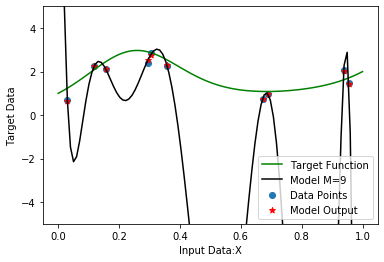
\includegraphics[width=1\textwidth]{M=9.png}\\
        (d) M=9
    \end{minipage}
    \label{fig:l}
\end{figure}

\begin{table}[h!]
\centering
 \begin{tabular}{|c|c|c|c|c|} 
 \hline
 Coefficient & M=1 & M=3 & M=6 & M=9 \\ [0.5ex] 
 \hline
 w_{0} & 2.02427      &  0.26983    &   -0.19544 &       24.55836\\
 w_{1} &-0.52891      & 19.56675    &   35.64357 &   -1450.29562\\
 w_{2} & 0.           &-49.13776    & -207.02909 &   28930.95753\\
 w_{3} & 0.           & 31.81886    &  734.13609 & -272882.72827\\
 w_{4} & 0.           &  0.         &-1569.81547 & 1411950.67306\\
 w_{5} & 0.           &  0.         & 1674.83597 &-4278106.07962\\
 w_{6} & 0.           &  0.         & -669.17919 & 7747617.91174\\
 w_{7} & 0.           &  0.         &    0.      &-8224348.55394\\
 w_{8} & 0.           &  0.         &    0.      & 4709126.58426\\
 w_{9} & 0.           &  0.         &    0.      &-1120968.27014\\
\hline
\end{tabular}
\caption{Table of Coefficients}
\end{table}
\newpage
\begin{equation}
   R.M.S Error=\sqrt{\frac{1}{D}*\sum_{i=1}^{D}(Y-Y_{reg})^2}  
\end{equation}

\begin{table}[h!]
\centering
 \begin{tabular}{|c|c|c|c|c|} 
 \hline
Degree(M) & M=1 & M=3 & M=6 & M=9 \\ [0.5ex] 
\hline
Training Error & 0.70471 &0.25507 &0.15938 &0.06622\\
Testing Error  &  0.57721& 0.45861& 0.69175&11.75728\\
\hline
\end{tabular}
\caption{Table of Errors for Linear Models on Training Data Set D of Size:10}
\end{table}
\begin{table}[h!]
\centering
 \begin{tabular}{|c|c|c|c|c|} 
 \hline
Degree(M) & M=1 & M=3 & M=6 & M=9 \\ [0.5ex] 
\hline
Training Error & 0.66484 &0.47411 &0.41564 &0.4144\\
Testing Error  & 0.56585 &0.4495  &0.40452 &0.40764\\
\hline
\end{tabular}
\caption{Table of Errors for Linear Models on Training Data Set D of Size:80}
\end{table}

\subproblem{b} As the Training Data Set Size(D) is increased gradually by 10 points beginning from D=10 till D=80 we see the following trends in the above four models:\\
\begin{figure}[!htb]
    \centering
    \begin{minipage}{0.49\textwidth}
        \centering
        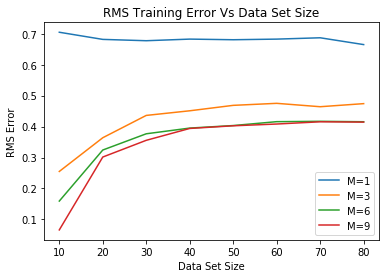
\includegraphics[width=1\textwidth]{ErrorTrain.png} \\
         
    \end{minipage}\hfill
    \begin{minipage}{0.49\textwidth}
        \centering
        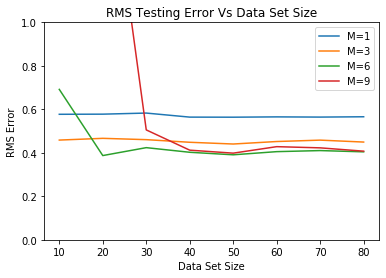
\includegraphics[width=1\textwidth]{ErrorTest.png}\\
    
    \end{minipage}
    \label{fig:l}
\end{figure}
\begin{itemize}
  \item  M=1: The linear model captures the data well in case of 10 points. But as the training data set increases it starts to under fit the data as the test error compared to other models starts increasing.
  \item  M=3: The cubic model is the best model for data set of size 10 as it has the least testing error. It continues to perform well even if the data set size is increased till 80 because it almost replicates the target function. 
  \item  M=6: The model has considerably high testing error and low training error which leads to over-fitting in the beginning. The model however starts giving accurate results as the data set size is increased.
  It in fact becomes best model for data set of size 80.
  \item M=9: From the above figure(d), Table of Coefficients and Table of Errors, it is clear that the polynomial of degree(M)=9 over-fits the 10 data points chosen as it has nearly zero training error and a huge testing error.
  However, as the Data Set size increases from 10 to 80 we see that training error gradually increases whereas the testing error drastically reduces. Hence the over-fit decreases as data set size increases.
\end{itemize}



\newpage
\bigskip
\subproblem{c}  It can be seen from Table 11 that the least test error is achieved for polynomial of degree M=6. Hence the Best Model for the Training Data Set of Size  D=80 is M=6.\\

\begin{figure}[!htb]
    \centering
    \begin{minipage}{0.49\textwidth}
        \centering
        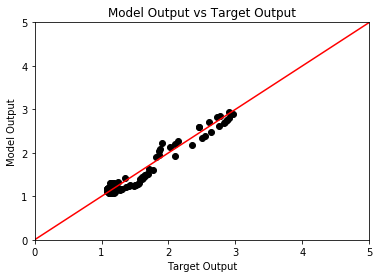
\includegraphics[width=1\textwidth]{T vs Y train.png} \\
         Training Data Set 
    \end{minipage}\hfill
    \begin{minipage}{0.49\textwidth}
        \centering
        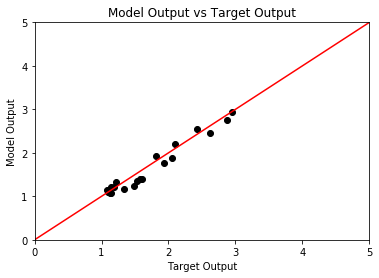
\includegraphics[width=1\textwidth]{T vs Y test.png}\\
         Testing Data Set
    \end{minipage}
    \label{fig:l}
\end{figure}
All the points lie very close to the $45^{o}$ red line. This implies that the model output values and the respective target value are almost the same. Points on the line are the ones where the model correctly predicts the target value. \\
\subproblem{d} RMS Error Plots:\\
\begin{figure}[!htb]
    \centering
    \begin{minipage}{0.49\textwidth}
        \centering
        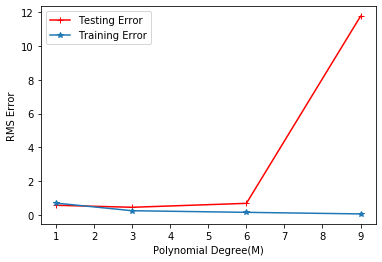
\includegraphics[width=1\textwidth]{D=10 RMS Error.png} \\
         Training Data Set of Size 10
    \end{minipage}\hfill
    \begin{minipage}{0.49\textwidth}
        \centering
        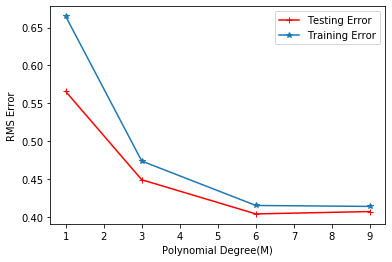
\includegraphics[width=1\textwidth]{D=80 RMS Error.png}\\
         Training Data Set of Size 80
    \end{minipage}
    \label{fig:l}
\end{figure}
 The R.M.S Error Tables 10 and 11 show values for the models under consideration. \\
\begin{itemize}
    \item Hence the best model for Data Set of 10 Points is the Cubic Model (M=3).
    \item The best model for Data  Set of 80 Points is the Polynomial Model with degree (M)=6.

\end{itemize}



\end{document} 
